\section{Scenarios}

This section contains four scenario's and how the architecture responds to them. The format is obtained from \cite{clemens}. The choices for scenario's were made on multiple factors:
\begin{enumerate}
\itemsep0em 
\item To demonstrate one of the key design decisions and the related trade-offs and sensitivity points (\ref{sec:failureb2b})
\item To indicate that some (implicit) design decisions are still open for discussion (\ref{sec:peakload},\ref{sec:privacy})
\item To test how the architecture responds to a change in an assumption and which components need to be modified (\ref{sec:bigdata})
\end{enumerate}

\subsection{Scenario: Failure in B2B/B2C} \label{sec:failureb2b}
\begin{tabularx}{\textwidth}{| l | X |}
  \hline
  \textbf{Scenario} & B2B - B2C decoupling \\
  \hline
  \textbf{Attribute} & Availability \\
  \hline
  \textbf{Environment} & Normal Operations \\
  \hline
  \textbf{Stimulus} & B2B or B2C failure \\
  \hline
  \textbf{Response} & Failure of either one does not influence the other. \\
  \hline
    &
    \begin{tabular}[t]{ | @{}| p{4cm} | l | l | l | l | @{} | }
      \hline
      \textbf{Architectural Decision} & \textbf{Sensitivity} & \textbf{Tradeoff} & \textbf{Risk} & \textbf{Non-risk} \\
      \hline
      Decoupling & S1 & T1 & & \\
      \hline
      Different API & S1 & T2 & & N1 \\
      \hline
    \end{tabular}
    \\
    &  T1: When both systems are decoupled and both access the same data store a tradoff is created. The performance of the B2C clients is directly linked to the performance of the B2B clients \newline
    T2: The API contains duplicate functionality hence redundant code might exist. This is a trade off between modifiability/maintainability because of the redundant code vs availability (one system crashes does not influence the other system). \newline
    N1: If the API was not split up as well then this would create a single point of failure as mentioned by the architecs. \newline
    S1: If the B2B and B2C systems  are in the same server and the server goes down, B2C and B2B will both go down. \\
  \hline
  \textbf{Reasoning} & Decoupling ensures, together with the different API, that if one the B2B or B2C module goes down, the other won't. \\
  \hline
  \textbf{Architecture Diagram} & The red API crashes. \\
   & 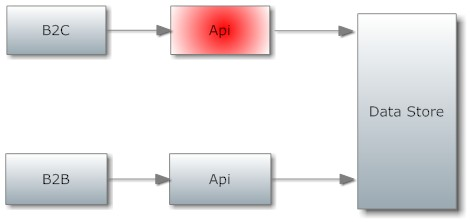
\includegraphics[width=250px]{scenario1} \\
  \hline
\end{tabularx}

\subsection{Scenario: Peak load on analytics module} \label{sec:peakload}

\begin{tabularx}{\textwidth}{| l | X |}
  \hline
  \textbf{Scenario} & Peak load on the analytics module \\
  \hline
  \textbf{Attribute} & Performance \\
  \hline
  \textbf{Environment} & Normal Operations \\
  \hline
  \textbf{Stimulus} & Recalculating ratings/reviews \\
  \hline
  \textbf{Response} & B2B latency <10 sec. \\
  \hline
    &
    \begin{tabular}[t]{ | @{}| p{4cm} | l | l | l | l | @{} | }
      \hline
      \textbf{Architectural Decision} & \textbf{Sensitivity} & \textbf{Tradeoff} & \textbf{Risk} & \textbf{Non-risk} \\
      \hline
      Recalculate 1/2 times a day (Implicit) & & & R1 & \\
      \hline
      B2B accesses analytics directly (Implicit) & & T1 & & \\
      \hline
    \end{tabular}
    \\
    & R1: Recalculating the final rating once or twice a day creates a major peak load on the analytics module and might lead to an unavailable analytics module for the B2B clients. \newline
    T1: B2B clients can directly access the analytics module, this gives the B2B clients the freedom to perform custom searches, but also leads to unavailability if the module is overburdend.\\
  \hline
  \textbf{Reasoning} & Recalculating on a time frame creates a massive peakload  which may lead to an undesirable response time when the B2B performs a custom search. \\
  \hline
  \textbf{Architecture Diagram} & Analytics module overloaded. \\
   & 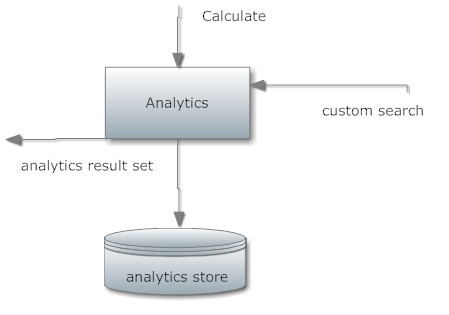
\includegraphics[width=300px]{scenario2} \\
  \hline
\end{tabularx}

\subsection{Scenario: Review privacy} \label{sec:privacy}

\begin{tabularx}{\textwidth}{| l | X |}
  \hline
  \textbf{Scenario} & Review Privacy \\
  \hline
  \textbf{Attribute} & Privacy \\
  \hline
  \textbf{Environment} & Normal Operations \\
  \hline
  \textbf{Stimulus} & User writes a review \\
  \hline
  \textbf{Response} & Anonymous review \\
  \hline
    &
    \begin{tabular}[t]{ | @{}| p{4cm} | l | l | l | l | @{} | }
      \hline
      \textbf{Architectural Decision} & \textbf{Sensitivity} & \textbf{Tradeoff} & \textbf{Risk} & \textbf{Non-risk} \\
      \hline
      Logged In & & & R1 & \\
      \hline
    \end{tabular}
    \\
    & R1: The anonymity of the user posting a review is not guaranteed.  \\
  \hline
  \textbf{Reasoning} & In the architecture it is not stated that a review will be shown anonymous or how anonimity of reviews is guaranteed. \\
  \hline
  \textbf{Architecture Diagram} & Anyone can see review details. \\
   & 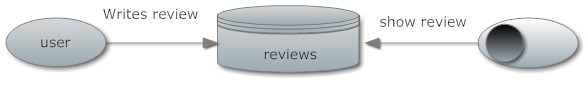
\includegraphics[width=300px]{scenario3} \\
  \hline
\end{tabularx}

\subsection{Scenario: Big data} \label{sec:bigdata}

\begin{tabularx}{\textwidth}{| l | X |}
  \hline
  \textbf{Scenario} & Big Data \\
  \hline
  \textbf{Attribute} & Performance, Availability \\
  \hline
  \textbf{Environment} & Normal Operations \\
  \hline
  \textbf{Stimulus} & Big Data input \\
  \hline
  \textbf{Response} & Handle all input without any loss of data. \\
  \hline
    &
    \begin{tabular}[t]{ | @{}| p{4cm} | l | l | l | l | @{} | }
      \hline
      \textbf{Architectural Decision} & \textbf{Sensitivity} & \textbf{Tradeoff} & \textbf{Risk} & \textbf{Non-risk} \\
      \hline
      ETL Adapters & & & & N1 \\
      \hline
      ETL Approaches & S1 & & & \\
      \hline
      Pipeline Structure & & & R1 & \\
      \hline
    \end{tabular}
    \\
    & S1: If it is Big data the system can not handle the input a choke point will occur in the pipe model. \newline
    N1: The modules in the ETL are independent and therefore easily modifiable. \newline
    R1: The \emph{Filter and Store} and \emph{Extract and apply} module process all reviews sequentially which is a risk regarding scalability \\
  \hline
  \textbf{Reasoning} & The pipeline structure won't be able to process large input sets of data (Big data).  \\
  \hline
  \textbf{Architecture Diagram}. \\
   & 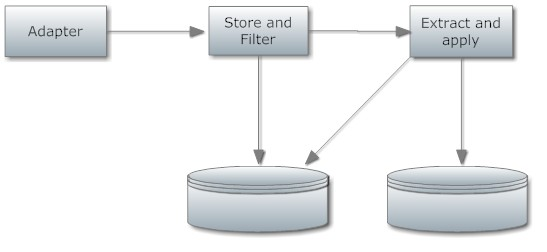
\includegraphics[width=300px]{scenario4} \\
  \hline
  \textbf{Notes} & The architectures note that \emph{a dramitacally higher number of reviews would choke the system}. It was therefore an explicit choice to not handle big data, however this scenario is valuable in that it identifies the components that need to be modified in order to make it more scalable. \\
  \hline
\end{tabularx}
